%%\textbf{Note that you may have multiple \texttt{{\textbackslash}include} statements here, e.g.\ one for each subsection.}\cofeBm{0.7}{1}{0}{3cm}{-1cm}
\chapter{Introduction}

\section{What is Hypernymy?} % why is this a non trivial problem
It is difficult to imagine a language which excludes generic terms or word classes entirely.  Such a language would be challenging to comprehend since a detailed definition of every word is required before a sentence or an utterance can be understood.  The definition needs to describe the word in terms of its base elements and would not be able to set it in a wider context of related words.  We imagine that communication in this hypothetical language would be a laborious task.  Translation would be an arduous, if not impossible, enterprise and our understanding of the world around us severely compromised.  It would be hard to imagine such a language being used on a day-to-day basis in today's highly-connected, globalised world.

Hypernymy is the semantic construct which matches words to their generic or \textit{superordinate} concepts.  From a young age, we learn several simple concepts such as \textit{dog} in terms of what they look like and how they act.  When reading about an unfamiliar dog breed – \textit{Pat, the family Labrador, barks and wags his tail when the doorbell rings} - we can immediately intuit that Pat is a dog and is more likely to be encountered in a park rather than a jungle even if we are entirely unfamiliar with the term \textit{Labrador}.  The same principle also applies to proper nouns; knowing that \textit{Donald Trump} is an \textit{American President} is very helpful when appraising a story about him in the press.  

Therefore, hypernymy describes the \textbf{is-a} relation between two words or phrases.  Ontologists go a step further and distinguish between the subclass relationship, which is used to relate concepts, and the instance which is employed to identify proper nouns \citep{miller1990introduction}.  Therefore \textit{heroine} is a \textbf{subclass} of \textit{woman} (all heroines are women) while \textit{Marie Curie} is an \textbf{instance} of a \textit{woman}.  Instances are normally terminal words in that there exists no other term in a word hierarchy which acts as sub-instance.  The notion of another woman claiming to be an instance of \textit{Marie Curie} is absurd.  Concepts, on the other hand, can have parent super-concepts as well as child sub-concepts.  A \textit{dog} is a \textit{mammal} and a \textit{terrier} is a \textit{dog}, from which we can also infer that a \textit{terrier} is a \textit{mammal}.

\section{Word Senses and Their Relationships}
We have introduced hypernymy as a semantic relationship between words but Jurafsky and Martin categorise hypernymy as a relation that binds two words senses together \citep{Jurafsky2009}.  A word is a discrete symbol and nothing in its composition (spelling or pronunciation) conveys any meaning.  Moreover, words can have an identical surface form and yet convey different meanings.  In linguistic semantics, this phenomenon is called homonymy.  Sometimes, the surface form can provide clues on the word’s meaning: \textit{Apple}, the proper noun is disambiguated from \textit{apple} the common noun, conveying the company and fruit senses of the word, even outside a wider textual context.  Of course, a common noun can be capitalised, as dictated by good grammatical form when the word is used at the beginning of a sentence.  In other cases, two different word senses can be lexically identical.  Consider for instance, the noun \textit{dog} in the domestic animal sense and the verb \textit{dog} which suggests the act of pursuit.  

A word’s surface form can be altered by morphological modifiers.  In the English language, the suffix \textbf{-s} often denotes a word’s plural form.  To distinguish among the potentially many word-forms of a word, the word’s lemma is cited.  The lemma can be understood as the word in its most unadorned form.  The lemma \textit{eat} can take the forms: \textit{eating}, \textit{eats}, \textit{ate}, \textit{eaten} amongst several others.  Lemmas do not have to be necessarily composed of a single word: \textit{Mick Jagger}, \textit{New York} and \textit{Pjazza Teatru Rjal} are all valid lemmas.

The word sense is a finer-grained label we attribute to words.  This allows us to distinguish between different semantic representations of the same word.  Jurafsky and Martin quote \textit{bank}, a well-known example \citep{Jurafsky2009}.  If we encounter \textit{bank} in the context of words like \textit{investment}, \textit{account} and \textit{custodial} we know we are referring to the financial institution.  However, the same word in the context of \textit{river}, \textit{mud} and \textit{south} suggest the sloping ground along the edge of a river.  In this example, \textit{bank} has two distinct word senses.  Apart from being a homonym, \textit{bank} is also polysemous because of the multiple repository senses of the word.  Thus \textit{blood bank} and \textit{sperm bank} are inherently different while still being semantically related to the repository-sense of \textit{bank} \citep{Jurafsky2009}.

Perhaps it is also important to note that a lemma may also refer to synonymous lexicalisations rather than the cited orthographic form of the word \citep{Jurafsky2009}.  In WordNet, a popular lexical resource discussed later, lemmas refer to the various lexicalisations of a \ac{synset} \citep{Miller1995}.  \textit{Car}, \textit{auto}, and \textit{automobile}, are different words which all mean \textit{car} in the four-wheeled, vehicle sense.  

The knowledge of a word’s sense can be a determining factor in finding its correct hypernym.  Given the word \textit{queen} and assuming it has been case-normalised, we could correctly propose \textit{monarch}, \textit{rock band}, \textit{chess piece} as equally correct hypernyms.   Knowledge of the exact sense would narrow down the hypernym candidates.  Now that we have clarified the important distinction between a word and a word sense, we can proceed to describe the various relationships that hold between word senses.  Henceforth, word sense and word may be used interchangeably.

Besides hypernymy, the main semantic relationships that will be mentioned in this text are \textbf{\textit{synonymy}}, \textbf{\textit{antonymy}}, \textbf{\textit{hyponymy}}, \textbf{\textit{co-hyponymy}}, and \textbf{\textit{meronymy}}.  After building a model designed to identify a particular semantic relationship - say hypernymy - between two words, researches often evaluate their solution’s performance by measuring how well it discriminates the target semantic relationship from other semantic relations \citep{shwartz2017siege, nguyen2017hierarchical, shwartz2016path}.  We briefly explain each in the following subsections.

\subsection{Synonymy}
Synonyms are words that are similar enough in meaning to be used interchangeably in a sentence without altering the sentence’s meaning.  We can replace \textit{automobile} with \textit{car} in \textit{I drove my car to work} and retain the same meaning although \textit{automobile} makes the sentence feel somewhat dated.  One could philosophically argue that no two words (lemmas) have the exact same meaning; there could be some nuance or colour that one word brings to a sentence which its synonym does not.  \textit{I invited my guest to sit on the couch} is semantically equivalent to \textit{I invited my guest to sit on the sofa} although the former could suggest that the narrator is American.  Synonymy is a symmetric relationship; therefore, \(synonym(x, y)\) and \(synonym(y, x)\) are equivalent.

\subsection{Antonymy}
Antonymy holds when a word has the opposite meaning of another word.  Antonymous words are often similar in every respect except for their magnitude or direction \citep{Jurafsky2009}.  For this reason, systems that attempt to identify semantic relations automatically can have a hard time at distinguishing antonymy from synonymy \citep{Jurafsky2009}.

\subsection{Hyponymy}
Hypernymy is an asymmetric relationship: \(hypernym(x, y) \nvDash hypernym(y, x)\).  Hyponymy is the inverse relationship of hypernymy which means that \(hypernym(x, y) \vDash hyponym(y, x)\).  Hypernymy holds if a language’s native speaker concurs that every \(x\) is a type of \(y\).  If this assertion is true, then we can also accept that \(x\) is an instance of \(y\).   

Hypernyms can themselves be hyponyms of more generic words featuring at higher levels of a word hierarchy.  The hypernymy relation is transitive and this property can be exploited to generate indirect hypernyms: given the tuples \((elephant, mammal)\) and \((mammal, animal)\), we can add a new hypernym word-pair \((elephant, animal)\).  The term \textbf{subordinate} is sometimes used an alternative word to hyponym whereas \textbf{superordinate} is an occasional substitute for hypernym.  These terms may be used interchangeably in this text.

\subsection{Co-hyponymy}
When two words share a common hypernym, they are related by co-hyponymy.  In contrast to synonyms, co-hyponyms can have very different meanings.  In Figure~\ref{fig:simple_taxon} from \citet{camacho2017we}, the lemmas \textit{dog} and  \textit{horse} represent different concepts but are considered co-hyponyms because they are both subordinates of \textit{mammal}.
\begin{figure}[ht!] % supposedly places it here ...
  \centering
  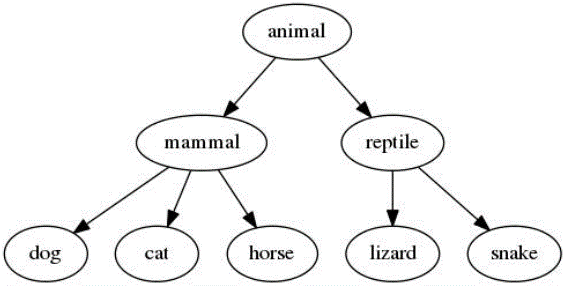
\includegraphics[width=0.6\linewidth]{images/simplified_animal_taxonomy.png}
  \caption{Simplified animal taxonomy.\index{Simplified animal taxonomy}}
  \label{fig:simple_taxon}
\end{figure}

\subsection{Meronymy}
Meronymy underlines the part-whole relationship of words.  A \textit{limb} is part of a \textit{body}; a \textit{wheel} is part of \textit{car}.  The inverse whole-part relationship is referred to as \textbf{\textit{holonymy}}; for example an \textit{engine} is composed of (one or several) \textit{piston}, \textit{valve}, \textit{crankshaft}, and so forth.

\section{Hypernymy Dependent Downstream Tasks}
Considering that hypernymy is at the heart of human comprehension, it is no surprise that the research community has been invested in the automatic identification of this semantic relation for more than twenty years \citep{camacho2018semeval}.  Hypernym identification is not solely done for its own sake.  In fact, it plays an important supporting role in tasks requiring a degree of logical inference.  These tasks are sometimes referred to as downstream tasks since they are dependent on hypernymy identification/discovery.  Examples include: question answering applications; automatic taxonomy construction; and lexical entailment.

\subsection{Question Answering}
In \citep{yang2017efficiently}, the authors construct a taxonomy of Microsoft products to power a system which can automatically answer technical questions. By linking instances such as \textit{Internet Explorer} to its superordinate \textit{browser}, the system will be able to retrieve documents pertaining to browsers when \textit{Internet Explorer} features in a question.

\subsection{Taxonomy Construction}
%% Need to provide more details here

\subsection{Lexical Entailment}
%% Need to provide more details here

\section{Limitation of Hypernymy Identification}
\citeauthor{camacho2017we} muses about the recent neglect of taxonomy construction in research, in favour of “simply” identifying hypernymy \citep{camacho2017we}.  He blames this primarily on the reliance on hand-crafted taxonomies for the evaluation of proposed solutions, which are expensive to procure.  On the other hand, hypernym detection is appreciably easier to evaluate due to the availability of several gold-standard datasets \citep{Baroni2011, santus2015evalution, weeds2014learning}.  Despite several developments in the area of hypernym detection, Camacho-Collados argues that merely determining whether hypernymy holds between a word-pair in a binary fashion is of limited use to downstream tasks \citep{camacho2017we}.  Consider the question “Which museums are open on Sunday in London” posed to a Question Answering system.  An effective system must be able to autonomously link various building instances with the \textit{museum} concept, before filtering those that are located in London and open on a Sunday.  Thus, the binary task is recast to a hypernym discovery problem whereby given a query term, a system is expected to emit a list of the word’s potential hypernyms.  To limit the problem’s search-space we normally require a vocabulary of candidate words often directly collected from the corpus/corpora.

The call to recast identification to discovery was answered by a SemEval committee who devised a shared task - SemEval 2018 Task 9 \footnote{https://competitions.codalab.org/competitions/17119} - that challenged participants to extract hypernyms directly from general-purpose and domain-specific corpora in English, Spanish and Italian.  This dissertation makes extensive use of the resources shipped with the task and employs techniques from the more performant submissions’ toolbox to fuel our exploration of hypernymy discovery. 

\section{Document Structure}
We first provide the background required to understand this task, and the experiments we carried out, by surveying the salient contributions made to the areas of hypernymy identification and discovery.   We start from the earliest handpicked pattern-based methods and see how even this relatively simple technique can be leveraged to induce a large, complex taxonomy.  

Dependency paths were later used to discover hypernym-containing patterns automatically.  Although never abandoned, pattern-centric approaches eventually gave way to distributional methods and \acl{VSM}s.  There are several \ac{VSM} flavours, each varying in terms of context type and feature weighting mechanism; we will introduce the main types used in the reviewed literature.  Several unsupervised metrics were developed that given the vector representation of two words, scored the likelihood that the words were bound by hypernymy based on their respective dimensional contexts.

When word embeddings burst onto the scene in 2013 \citep{mikolov2013distributed}, supervised methods involving various combinations of the hyponym and hypernym vector embeddings fed into a classifier acquired outstanding results in the hypernym identification binary task.  Closer inspection by researchers sceptical about these results underscored these methods’ proneness to overfitting the training data. In doing so, they shone a light on the limitation of the identification task and encouraged the NLP research community to recast identification to hypernym discovery.  We then move on to a variant of supervised learning which attempts to learn a linear projection learning matrix which when applied to a hyponym vector, yields a vector close to its hypernym.  We decided to focus particularly on this method in our experiments, considering their relative success in generating hypernyms.  
We close the background chapter by reviewing the SemEval 2018 Task 9 shared task \citep{camacho2018semeval}, concentrating on the methodology used to create the training and testing datasets which were part automated and part crowd-sourced.  Setting aside the popular precision/recall/\(F1\) evaluation measures, the task’s organisers propose a new set of metrics, borrowed from \ac{IR} that are suited to the ranking nature of the problem.  Finally, we examine the submitted models focusing on those which peruse of projection learning techniques to propose hypernyms for the given candidate terms.
